\documentclass[1p]{elsarticle_modified}
%\bibliographystyle{elsarticle-num}

%\usepackage[colorlinks]{hyperref}
%\usepackage{abbrmath_seonhwa} %\Abb, \Ascr, \Acal ,\Abf, \Afrak
\usepackage{amsfonts}
\usepackage{amssymb}
\usepackage{amsmath}
\usepackage{amsthm}
\usepackage{scalefnt}
\usepackage{amsbsy}
\usepackage{kotex}
\usepackage{caption}
\usepackage{subfig}
\usepackage{color}
\usepackage{graphicx}
\usepackage{xcolor} %% white, black, red, green, blue, cyan, magenta, yellow
\usepackage{float}
\usepackage{setspace}
\usepackage{hyperref}

\usepackage{tikz}
\usetikzlibrary{arrows}

\usepackage{multirow}
\usepackage{array} % fixed length table
\usepackage{hhline}

%%%%%%%%%%%%%%%%%%%%%
\makeatletter
\renewcommand*\env@matrix[1][\arraystretch]{%
	\edef\arraystretch{#1}%
	\hskip -\arraycolsep
	\let\@ifnextchar\new@ifnextchar
	\array{*\c@MaxMatrixCols c}}
\makeatother %https://tex.stackexchange.com/questions/14071/how-can-i-increase-the-line-spacing-in-a-matrix
%%%%%%%%%%%%%%%

\usepackage[normalem]{ulem}

\newcommand{\msout}[1]{\ifmmode\text{\sout{\ensuremath{#1}}}\else\sout{#1}\fi}
%SOURCE: \msout is \stkout macro in https://tex.stackexchange.com/questions/20609/strikeout-in-math-mode

\newcommand{\cancel}[1]{
	\ifmmode
	{\color{red}\msout{#1}}
	\else
	{\color{red}\sout{#1}}
	\fi
}

\newcommand{\add}[1]{
	{\color{blue}\uwave{#1}}
}

\newcommand{\replace}[2]{
	\ifmmode
	{\color{red}\msout{#1}}{\color{blue}\uwave{#2}}
	\else
	{\color{red}\sout{#1}}{\color{blue}\uwave{#2}}
	\fi
}

\newcommand{\Sol}{\mathcal{S}} %segment
\newcommand{\D}{D} %diagram
\newcommand{\A}{\mathcal{A}} %arc


%%%%%%%%%%%%%%%%%%%%%%%%%%%%%5 test

\def\sl{\operatorname{\textup{SL}}(2,\Cbb)}
\def\psl{\operatorname{\textup{PSL}}(2,\Cbb)}
\def\quan{\mkern 1mu \triangleright \mkern 1mu}

\theoremstyle{definition}
\newtheorem{thm}{Theorem}[section]
\newtheorem{prop}[thm]{Proposition}
\newtheorem{lem}[thm]{Lemma}
\newtheorem{ques}[thm]{Question}
\newtheorem{cor}[thm]{Corollary}
\newtheorem{defn}[thm]{Definition}
\newtheorem{exam}[thm]{Example}
\newtheorem{rmk}[thm]{Remark}
\newtheorem{alg}[thm]{Algorithm}

\newcommand{\I}{\sqrt{-1}}
\begin{document}

%\begin{frontmatter}
%
%\title{Boundary parabolic representations of knots up to 8 crossings}
%
%%% Group authors per affiliation:
%\author{Yunhi Cho} 
%\address{Department of Mathematics, University of Seoul, Seoul, Korea}
%\ead{yhcho@uos.ac.kr}
%
%
%\author{Seonhwa Kim} %\fnref{s_kim}}
%\address{Center for Geometry and Physics, Institute for Basic Science, Pohang, 37673, Korea}
%\ead{ryeona17@ibs.re.kr}
%
%\author{Hyuk Kim}
%\address{Department of Mathematical Sciences, Seoul National University, Seoul 08826, Korea}
%\ead{hyukkim@snu.ac.kr}
%
%\author{Seokbeom Yoon}
%\address{Department of Mathematical Sciences, Seoul National University, Seoul, 08826,  Korea}
%\ead{sbyoon15@snu.ac.kr}
%
%\begin{abstract}
%We find all boundary parabolic representation of knots up to 8 crossings.
%
%\end{abstract}
%\begin{keyword}
%    \MSC[2010] 57M25 
%\end{keyword}
%
%\end{frontmatter}

%\linenumbers
%\tableofcontents
%
\newcommand\colored[1]{\textcolor{white}{\rule[-0.35ex]{0.8em}{1.4ex}}\kern-0.8em\color{red} #1}%
%\newcommand\colored[1]{\textcolor{white}{ #1}\kern-2.17ex	\textcolor{white}{ #1}\kern-1.81ex	\textcolor{white}{ #1}\kern-2.15ex\color{red}#1	}

{\Large $\underline{12a_{1115}~(K12a_{1115})}$}

\setlength{\tabcolsep}{10pt}
\renewcommand{\arraystretch}{1.6}
\vspace{1cm}\begin{tabular}{m{100pt}>{\centering\arraybackslash}m{274pt}}
\multirow{5}{120pt}{
	\centering
	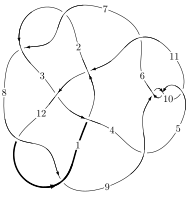
\includegraphics[width=112pt]{../../../GIT/diagram.site/Diagrams/png/1916_12a_1115.png}\\
\ \ \ A knot diagram\footnotemark}&
\allowdisplaybreaks
\textbf{Linearized knot diagam} \\
\cline{2-2}
 &
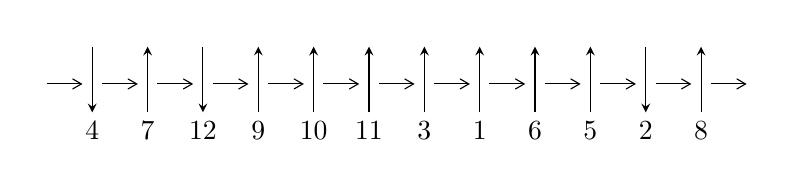
\begin{tikzpicture}[x=20pt, y=17pt]
	% nodes
	\node (C0) at (0, 0) {};
	\node (C1) at (1, 0) {};
	\node (C1U) at (1, +1) {};
	\node (C1D) at (1, -1) {4};

	\node (C2) at (2, 0) {};
	\node (C2U) at (2, +1) {};
	\node (C2D) at (2, -1) {7};

	\node (C3) at (3, 0) {};
	\node (C3U) at (3, +1) {};
	\node (C3D) at (3, -1) {12};

	\node (C4) at (4, 0) {};
	\node (C4U) at (4, +1) {};
	\node (C4D) at (4, -1) {9};

	\node (C5) at (5, 0) {};
	\node (C5U) at (5, +1) {};
	\node (C5D) at (5, -1) {10};

	\node (C6) at (6, 0) {};
	\node (C6U) at (6, +1) {};
	\node (C6D) at (6, -1) {11};

	\node (C7) at (7, 0) {};
	\node (C7U) at (7, +1) {};
	\node (C7D) at (7, -1) {3};

	\node (C8) at (8, 0) {};
	\node (C8U) at (8, +1) {};
	\node (C8D) at (8, -1) {1};

	\node (C9) at (9, 0) {};
	\node (C9U) at (9, +1) {};
	\node (C9D) at (9, -1) {6};

	\node (C10) at (10, 0) {};
	\node (C10U) at (10, +1) {};
	\node (C10D) at (10, -1) {5};

	\node (C11) at (11, 0) {};
	\node (C11U) at (11, +1) {};
	\node (C11D) at (11, -1) {2};

	\node (C12) at (12, 0) {};
	\node (C12U) at (12, +1) {};
	\node (C12D) at (12, -1) {8};
	\node (C13) at (13, 0) {};

	% arrows
	\draw[->,>={angle 60}]
	(C0) edge (C1) (C1) edge (C2) (C2) edge (C3) (C3) edge (C4) (C4) edge (C5) (C5) edge (C6) (C6) edge (C7) (C7) edge (C8) (C8) edge (C9) (C9) edge (C10) (C10) edge (C11) (C11) edge (C12) (C12) edge (C13) ;	\draw[->,>=stealth]
	(C1U) edge (C1D) (C2D) edge (C2U) (C3U) edge (C3D) (C4D) edge (C4U) (C5D) edge (C5U) (C6D) edge (C6U) (C7D) edge (C7U) (C8D) edge (C8U) (C9D) edge (C9U) (C10D) edge (C10U) (C11U) edge (C11D) (C12D) edge (C12U) ;
	\end{tikzpicture} \\
\hhline{~~} \\& 
\textbf{Solving Sequence} \\ \cline{2-2} 
 &
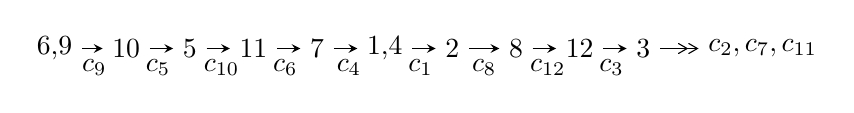
\begin{tikzpicture}[x=23pt, y=7pt]
	% node
	\node (A0) at (-1/8, 0) {6,9};
	\node (A1) at (1, 0) {10};
	\node (A2) at (2, 0) {5};
	\node (A3) at (3, 0) {11};
	\node (A4) at (4, 0) {7};
	\node (A5) at (81/16, 0) {1,4};
	\node (A6) at (49/8, 0) {2};
	\node (A7) at (57/8, 0) {8};
	\node (A8) at (65/8, 0) {12};
	\node (A9) at (73/8, 0) {3};
	\node (C1) at (1/2, -1) {$c_{9}$};
	\node (C2) at (3/2, -1) {$c_{5}$};
	\node (C3) at (5/2, -1) {$c_{10}$};
	\node (C4) at (7/2, -1) {$c_{6}$};
	\node (C5) at (9/2, -1) {$c_{4}$};
	\node (C6) at (45/8, -1) {$c_{1}$};
	\node (C7) at (53/8, -1) {$c_{8}$};
	\node (C8) at (61/8, -1) {$c_{12}$};
	\node (C9) at (69/8, -1) {$c_{3}$};
	\node (A10) at (11, 0) {$c_{2},c_{7},c_{11}$};

	% edge
	\draw[->,>=stealth]	
	(A0) edge (A1) (A1) edge (A2) (A2) edge (A3) (A3) edge (A4) (A4) edge (A5) (A5) edge (A6) (A6) edge (A7) (A7) edge (A8) (A8) edge (A9) ;
	\draw[->>,>={angle 60}]	
	(A9) edge (A10);
\end{tikzpicture} \\ 

\end{tabular} \\

\footnotetext{
The image of knot diagram is generated by the software ``\textbf{Draw programme}" developed by Andrew Bartholomew(\url{http://www.layer8.co.uk/maths/draw/index.htm\#Running-draw}), where we modified some parts for our purpose(\url{https://github.com/CATsTAILs/LinksPainter}).
}\phantom \\ \newline 
\centering \textbf{Ideals for irreducible components\footnotemark of $X_{\text{par}}$} 
 
\begin{align*}
I^u_{1}&=\langle 
15 u^{35}+68 u^{34}+\cdots+2 b-38,\;-9 u^{35}-36 u^{34}+\cdots+4 a+72,\;u^{36}+6 u^{35}+\cdots-10 u-4\rangle \\
I^u_{2}&=\langle 
-415484 u^5 a^3+374659 u^5 a^2+\cdots+1141045 a+3493341,\;u^5 a^3- u^5 a^2+\cdots-62 a+184,\\
\phantom{I^u_{2}}&\phantom{= \langle  }u^6+3 u^4+u^3+2 u^2+2 u-1\rangle \\
I^u_{3}&=\langle 
u^{16}+u^{15}+\cdots+b+2,\;-2 u^{17}-2 u^{16}+\cdots+a-2,\;u^{18}+u^{17}+\cdots+2 u+1\rangle \\
I^u_{4}&=\langle 
-352079058 u^9 a^3-279641663 u^9 a^2+\cdots+597636419 a-889033224,\\
\phantom{I^u_{4}}&\phantom{= \langle  }2 u^9 a^3+3 u^9 a^2+\cdots+2 a+4,\;u^{10}- u^9+4 u^8-4 u^7+6 u^6-6 u^5+3 u^4-3 u^3+1\rangle \\
\\
\end{align*}
\raggedright * 4 irreducible components of $\dim_{\mathbb{C}}=0$, with total 118 representations.\\
\footnotetext{All coefficients of polynomials are rational numbers. But the coefficients are sometimes approximated in decimal forms when there is not enough margin.}
\newpage
\renewcommand{\arraystretch}{1}
\centering \section*{I. $I^u_{1}= \langle 15 u^{35}+68 u^{34}+\cdots+2 b-38,\;-9 u^{35}-36 u^{34}+\cdots+4 a+72,\;u^{36}+6 u^{35}+\cdots-10 u-4 \rangle$}
\flushleft \textbf{(i) Arc colorings}\\
\begin{tabular}{m{7pt} m{180pt} m{7pt} m{180pt} }
\flushright $a_{6}=$&$\begin{pmatrix}0\\u\end{pmatrix}$ \\
\flushright $a_{9}=$&$\begin{pmatrix}1\\0\end{pmatrix}$ \\
\flushright $a_{10}=$&$\begin{pmatrix}1\\- u^2\end{pmatrix}$ \\
\flushright $a_{5}=$&$\begin{pmatrix}- u\\u^3+u\end{pmatrix}$ \\
\flushright $a_{11}=$&$\begin{pmatrix}u^2+1\\- u^4-2 u^2\end{pmatrix}$ \\
\flushright $a_{7}=$&$\begin{pmatrix}u^5+2 u^3+u\\- u^7-3 u^5-2 u^3+u\end{pmatrix}$ \\
\flushright $a_{1}=$&$\begin{pmatrix}\frac{9}{4} u^{35}+9 u^{34}+\cdots-\frac{79}{4} u-18\\-\frac{15}{2} u^{35}-34 u^{34}+\cdots+\frac{41}{2} u+19\end{pmatrix}$ \\
\flushright $a_{4}=$&$\begin{pmatrix}- u^3-2 u\\u^3+u\end{pmatrix}$ \\
\flushright $a_{2}=$&$\begin{pmatrix}\frac{49}{4} u^{35}+56 u^{34}+\cdots-\frac{247}{4} u-66\\-\frac{35}{2} u^{35}-84 u^{34}+\cdots+\frac{113}{2} u+49\end{pmatrix}$ \\
\flushright $a_{8}=$&$\begin{pmatrix}-4 u^{35}-\frac{43}{2} u^{34}+\cdots+25 u+\frac{27}{2}\\\frac{5}{2} u^{35}+15 u^{34}+\cdots-\frac{57}{2} u-18\end{pmatrix}$ \\
\flushright $a_{12}=$&$\begin{pmatrix}\frac{7}{2} u^{35}+\frac{33}{2} u^{34}+\cdots-\frac{43}{2} u-\frac{45}{2}\\-\frac{9}{2} u^{35}-21 u^{34}+\cdots+\frac{23}{2} u+14\end{pmatrix}$ \\
\flushright $a_{3}=$&$\begin{pmatrix}\frac{1}{4} u^{35}+3 u^{34}+\cdots-\frac{31}{4} u-8\\\frac{1}{2} u^{35}+u^{34}+\cdots-\frac{3}{2} u+3\end{pmatrix}$\\&\end{tabular}
\flushleft \textbf{(ii) Obstruction class $= -1$}\\~\\
\flushleft \textbf{(iii) Cusp Shapes $= 13 u^{35}+78 u^{34}+\cdots-156 u-78$}\\~\\
\newpage\renewcommand{\arraystretch}{1}
\flushleft \textbf{(iv) u-Polynomials at the component}\newline \\
\begin{tabular}{m{50pt}|m{274pt}}
Crossings & \hspace{64pt}u-Polynomials at each crossing \\
\hline $$\begin{aligned}c_{1},c_{11}\end{aligned}$$&$\begin{aligned}
&u^{36}+3 u^{35}+\cdots+10 u-1
\end{aligned}$\\
\hline $$\begin{aligned}c_{2},c_{7},c_{8}\\c_{12}\end{aligned}$$&$\begin{aligned}
&u^{36}+u^{35}+\cdots-4 u^2+1
\end{aligned}$\\
\hline $$\begin{aligned}c_{3}\end{aligned}$$&$\begin{aligned}
&u^{36}+36 u^{35}+\cdots-851968 u-65536
\end{aligned}$\\
\hline $$\begin{aligned}c_{4},c_{6}\end{aligned}$$&$\begin{aligned}
&u^{36}+6 u^{35}+\cdots-3456 u-712
\end{aligned}$\\
\hline $$\begin{aligned}c_{5},c_{9},c_{10}\end{aligned}$$&$\begin{aligned}
&u^{36}-6 u^{35}+\cdots+10 u-4
\end{aligned}$\\
\hline
\end{tabular}\\~\\
\newpage\renewcommand{\arraystretch}{1}
\flushleft \textbf{(v) Riley Polynomials at the component}\newline \\
\begin{tabular}{m{50pt}|m{274pt}}
Crossings & \hspace{64pt}Riley Polynomials at each crossing \\
\hline $$\begin{aligned}c_{1},c_{11}\end{aligned}$$&$\begin{aligned}
&y^{36}+13 y^{35}+\cdots-108 y+1
\end{aligned}$\\
\hline $$\begin{aligned}c_{2},c_{7},c_{8}\\c_{12}\end{aligned}$$&$\begin{aligned}
&y^{36}-31 y^{35}+\cdots-8 y+1
\end{aligned}$\\
\hline $$\begin{aligned}c_{3}\end{aligned}$$&$\begin{aligned}
&y^{36}+8 y^{35}+\cdots-81604378624 y+4294967296
\end{aligned}$\\
\hline $$\begin{aligned}c_{4},c_{6}\end{aligned}$$&$\begin{aligned}
&y^{36}-26 y^{35}+\cdots-1429120 y+506944
\end{aligned}$\\
\hline $$\begin{aligned}c_{5},c_{9},c_{10}\end{aligned}$$&$\begin{aligned}
&y^{36}+30 y^{35}+\cdots-108 y+16
\end{aligned}$\\
\hline
\end{tabular}\\~\\
\newpage\flushleft \textbf{(vi) Complex Volumes and Cusp Shapes}
$$\begin{array}{c|c|c}  
\text{Solutions to }I^u_{1}& \I (\text{vol} + \sqrt{-1}CS) & \text{Cusp shape}\\
 \hline 
\begin{aligned}
u &= -0.918601 + 0.135473 I \\
a &= -2.16683 - 0.71703 I \\
b &= \phantom{-}1.310650 - 0.016930 I\end{aligned}
 & \phantom{-}11.86120 - 2.65850 I & \phantom{-}16.0062 + 3.1622 I \\ \hline\begin{aligned}
u &= -0.918601 - 0.135473 I \\
a &= -2.16683 + 0.71703 I \\
b &= \phantom{-}1.310650 + 0.016930 I\end{aligned}
 & \phantom{-}11.86120 + 2.65850 I & \phantom{-}16.0062 - 3.1622 I \\ \hline\begin{aligned}
u &= -0.886777 + 0.100899 I \\
a &= \phantom{-}2.80734 + 0.39802 I \\
b &= -1.51502 + 0.47144 I\end{aligned}
 & \phantom{-}13.5026 - 12.5111 I & \phantom{-}13.4715 + 6.4902 I \\ \hline\begin{aligned}
u &= -0.886777 - 0.100899 I \\
a &= \phantom{-}2.80734 - 0.39802 I \\
b &= -1.51502 - 0.47144 I\end{aligned}
 & \phantom{-}13.5026 + 12.5111 I & \phantom{-}13.4715 - 6.4902 I \\ \hline\begin{aligned}
u &= \phantom{-}0.582328 + 0.632591 I \\
a &= \phantom{-}1.065630 - 0.902416 I \\
b &= -1.302410 + 0.256154 I\end{aligned}
 & \phantom{-}6.20237 - 3.57524 I & \phantom{-}13.30271 + 2.91674 I \\ \hline\begin{aligned}
u &= \phantom{-}0.582328 - 0.632591 I \\
a &= \phantom{-}1.065630 + 0.902416 I \\
b &= -1.302410 - 0.256154 I\end{aligned}
 & \phantom{-}6.20237 + 3.57524 I & \phantom{-}13.30271 - 2.91674 I \\ \hline\begin{aligned}
u &= -0.805953 + 0.027041 I \\
a &= -0.345526 + 0.596121 I \\
b &= \phantom{-}0.024838 - 0.844400 I\end{aligned}
 & \phantom{-}3.39332 - 2.17431 I & \phantom{-}8.53831 + 3.28500 I \\ \hline\begin{aligned}
u &= -0.805953 - 0.027041 I \\
a &= -0.345526 - 0.596121 I \\
b &= \phantom{-}0.024838 + 0.844400 I\end{aligned}
 & \phantom{-}3.39332 + 2.17431 I & \phantom{-}8.53831 - 3.28500 I \\ \hline\begin{aligned}
u &= \phantom{-}0.642311 + 0.449784 I \\
a &= -1.75182 + 0.80743 I \\
b &= \phantom{-}1.347300 + 0.355724 I\end{aligned}
 & \phantom{-}6.72630 + 7.92579 I & \phantom{-}12.1583 - 8.1491 I \\ \hline\begin{aligned}
u &= \phantom{-}0.642311 - 0.449784 I \\
a &= -1.75182 - 0.80743 I \\
b &= \phantom{-}1.347300 - 0.355724 I\end{aligned}
 & \phantom{-}6.72630 - 7.92579 I & \phantom{-}12.1583 + 8.1491 I\\
 \hline 
 \end{array}$$\newpage$$\begin{array}{c|c|c}  
\text{Solutions to }I^u_{1}& \I (\text{vol} + \sqrt{-1}CS) & \text{Cusp shape}\\
 \hline 
\begin{aligned}
u &= -0.501660 + 1.136970 I \\
a &= \phantom{-}1.286290 + 0.341993 I \\
b &= -1.326480 + 0.043785 I\end{aligned}
 & \phantom{-}8.78940 - 2.36934 I & \phantom{-}14.1647 + 0. I\phantom{ +0.000000I} \\ \hline\begin{aligned}
u &= -0.501660 - 1.136970 I \\
a &= \phantom{-}1.286290 - 0.341993 I \\
b &= -1.326480 - 0.043785 I\end{aligned}
 & \phantom{-}8.78940 + 2.36934 I & \phantom{-}14.1647 + 0. I\phantom{ +0.000000I} \\ \hline\begin{aligned}
u &= -0.452030 + 1.175710 I \\
a &= -1.302930 - 0.542898 I \\
b &= \phantom{-}1.50606 + 0.43598 I\end{aligned}
 & \phantom{-}10.20350 + 7.73445 I & \phantom{-0.000000 } 0 \\ \hline\begin{aligned}
u &= -0.452030 - 1.175710 I \\
a &= -1.302930 + 0.542898 I \\
b &= \phantom{-}1.50606 - 0.43598 I\end{aligned}
 & \phantom{-}10.20350 - 7.73445 I & \phantom{-0.000000 } 0 \\ \hline\begin{aligned}
u &= -0.084827 + 1.288850 I \\
a &= -0.259022 - 0.468223 I \\
b &= \phantom{-}0.470070 - 0.345741 I\end{aligned}
 & -3.34519 - 1.63537 I & \phantom{-0.000000 } 0 \\ \hline\begin{aligned}
u &= -0.084827 - 1.288850 I \\
a &= -0.259022 + 0.468223 I \\
b &= \phantom{-}0.470070 + 0.345741 I\end{aligned}
 & -3.34519 + 1.63537 I & \phantom{-0.000000 } 0 \\ \hline\begin{aligned}
u &= \phantom{-}0.235443 + 1.273080 I \\
a &= -1.35454 + 1.10271 I \\
b &= \phantom{-}0.631652 + 0.250784 I\end{aligned}
 & -4.21138 + 3.05086 I & \phantom{-0.000000 } 0 \\ \hline\begin{aligned}
u &= \phantom{-}0.235443 - 1.273080 I \\
a &= -1.35454 - 1.10271 I \\
b &= \phantom{-}0.631652 - 0.250784 I\end{aligned}
 & -4.21138 - 3.05086 I & \phantom{-0.000000 } 0 \\ \hline\begin{aligned}
u &= -0.349327 + 1.249240 I \\
a &= -0.335653 - 0.135529 I \\
b &= -0.108783 - 0.819825 I\end{aligned}
 & -0.38230 - 1.98485 I & \phantom{-0.000000 } 0 \\ \hline\begin{aligned}
u &= -0.349327 - 1.249240 I \\
a &= -0.335653 + 0.135529 I \\
b &= -0.108783 + 0.819825 I\end{aligned}
 & -0.38230 + 1.98485 I & \phantom{-0.000000 } 0\\
 \hline 
 \end{array}$$\newpage$$\begin{array}{c|c|c}  
\text{Solutions to }I^u_{1}& \I (\text{vol} + \sqrt{-1}CS) & \text{Cusp shape}\\
 \hline 
\begin{aligned}
u &= \phantom{-}0.071803 + 1.298360 I \\
a &= -0.143695 + 1.377620 I \\
b &= -0.296292 + 0.618271 I\end{aligned}
 & -5.96094 + 1.93016 I & \phantom{-0.000000 } 0 \\ \hline\begin{aligned}
u &= \phantom{-}0.071803 - 1.298360 I \\
a &= -0.143695 - 1.377620 I \\
b &= -0.296292 - 0.618271 I\end{aligned}
 & -5.96094 - 1.93016 I & \phantom{-0.000000 } 0 \\ \hline\begin{aligned}
u &= -0.358553 + 1.289720 I \\
a &= \phantom{-}0.899152 + 0.306766 I \\
b &= \phantom{-}0.043249 + 0.867682 I\end{aligned}
 & -0.71095 - 6.36900 I & \phantom{-0.000000 } 0 \\ \hline\begin{aligned}
u &= -0.358553 - 1.289720 I \\
a &= \phantom{-}0.899152 - 0.306766 I \\
b &= \phantom{-}0.043249 - 0.867682 I\end{aligned}
 & -0.71095 + 6.36900 I & \phantom{-0.000000 } 0 \\ \hline\begin{aligned}
u &= \phantom{-}0.610254\phantom{ +0.000000I} \\
a &= \phantom{-}2.40590\phantom{ +0.000000I} \\
b &= -0.572689\phantom{ +0.000000I}\end{aligned}
 & -0.250744\phantom{ +0.000000I} & \phantom{-}18.0910\phantom{ +0.000000I} \\ \hline\begin{aligned}
u &= -0.399118 + 1.345260 I \\
a &= -1.62048 - 1.69722 I \\
b &= \phantom{-}1.51341 - 0.49950 I\end{aligned}
 & \phantom{-}8.9652 - 17.1215 I & \phantom{-0.000000 } 0 \\ \hline\begin{aligned}
u &= -0.399118 - 1.345260 I \\
a &= -1.62048 + 1.69722 I \\
b &= \phantom{-}1.51341 + 0.49950 I\end{aligned}
 & \phantom{-}8.9652 + 17.1215 I & \phantom{-0.000000 } 0 \\ \hline\begin{aligned}
u &= \phantom{-}0.18895 + 1.40967 I \\
a &= \phantom{-}0.307536 - 1.289560 I \\
b &= -1.319040 - 0.457572 I\end{aligned}
 & \phantom{-}0.76991 + 10.74510 I & \phantom{-0.000000 } 0 \\ \hline\begin{aligned}
u &= \phantom{-}0.18895 - 1.40967 I \\
a &= \phantom{-}0.307536 + 1.289560 I \\
b &= -1.319040 + 0.457572 I\end{aligned}
 & \phantom{-}0.76991 - 10.74510 I & \phantom{-0.000000 } 0 \\ \hline\begin{aligned}
u &= -0.41508 + 1.37015 I \\
a &= \phantom{-}1.04177 + 1.33272 I \\
b &= -1.284840 + 0.058721 I\end{aligned}
 & \phantom{-}7.13077 - 7.43744 I & \phantom{-0.000000 } 0\\
 \hline 
 \end{array}$$\newpage$$\begin{array}{c|c|c}  
\text{Solutions to }I^u_{1}& \I (\text{vol} + \sqrt{-1}CS) & \text{Cusp shape}\\
 \hline 
\begin{aligned}
u &= -0.41508 - 1.37015 I \\
a &= \phantom{-}1.04177 - 1.33272 I \\
b &= -1.284840 - 0.058721 I\end{aligned}
 & \phantom{-}7.13077 + 7.43744 I & \phantom{-0.000000 } 0 \\ \hline\begin{aligned}
u &= \phantom{-}0.09158 + 1.50603 I \\
a &= \phantom{-}0.067556 + 0.267829 I \\
b &= \phantom{-}1.171500 - 0.194024 I\end{aligned}
 & -0.95947 - 1.45291 I & \phantom{-0.000000 } 0 \\ \hline\begin{aligned}
u &= \phantom{-}0.09158 - 1.50603 I \\
a &= \phantom{-}0.067556 - 0.267829 I \\
b &= \phantom{-}1.171500 + 0.194024 I\end{aligned}
 & -0.95947 + 1.45291 I & \phantom{-0.000000 } 0 \\ \hline\begin{aligned}
u &= -0.389978\phantom{ +0.000000I} \\
a &= \phantom{-}0.839038\phantom{ +0.000000I} \\
b &= -0.338534\phantom{ +0.000000I}\end{aligned}
 & \phantom{-}0.631815\phantom{ +0.000000I} & \phantom{-}16.0810\phantom{ +0.000000I} \\ \hline\begin{aligned}
u &= \phantom{-}0.249379 + 0.255614 I \\
a &= \phantom{-}0.432749 - 1.105430 I \\
b &= \phantom{-}0.089749 - 0.497899 I\end{aligned}
 & -1.30214 + 0.83943 I & -2.00109 - 3.97156 I \\ \hline\begin{aligned}
u &= \phantom{-}0.249379 - 0.255614 I \\
a &= \phantom{-}0.432749 + 1.105430 I \\
b &= \phantom{-}0.089749 + 0.497899 I\end{aligned}
 & -1.30214 - 0.83943 I & -2.00109 + 3.97156 I\\
 \hline 
 \end{array}$$\newpage\newpage\renewcommand{\arraystretch}{1}
\centering \section*{II. $I^u_{2}= \langle -4.15\times10^{5} a^{3} u^{5}+3.75\times10^{5} a^{2} u^{5}+\cdots+1.14\times10^{6} a+3.49\times10^{6},\;u^5 a^3- u^5 a^2+\cdots-62 a+184,\;u^6+3 u^4+u^3+2 u^2+2 u-1 \rangle$}
\flushleft \textbf{(i) Arc colorings}\\
\begin{tabular}{m{7pt} m{180pt} m{7pt} m{180pt} }
\flushright $a_{6}=$&$\begin{pmatrix}0\\u\end{pmatrix}$ \\
\flushright $a_{9}=$&$\begin{pmatrix}1\\0\end{pmatrix}$ \\
\flushright $a_{10}=$&$\begin{pmatrix}1\\- u^2\end{pmatrix}$ \\
\flushright $a_{5}=$&$\begin{pmatrix}- u\\u^3+u\end{pmatrix}$ \\
\flushright $a_{11}=$&$\begin{pmatrix}u^2+1\\- u^4-2 u^2\end{pmatrix}$ \\
\flushright $a_{7}=$&$\begin{pmatrix}u^5+2 u^3+u\\u^4+2 u^2\end{pmatrix}$ \\
\flushright $a_{1}=$&$\begin{pmatrix}a\\0.126898 a^{3} u^{5}-0.114429 a^{2} u^{5}+\cdots-0.348501 a-1.06694\end{pmatrix}$ \\
\flushright $a_{4}=$&$\begin{pmatrix}- u^3-2 u\\u^3+u\end{pmatrix}$ \\
\flushright $a_{2}=$&$\begin{pmatrix}-0.00312508 a^{3} u^{5}+0.0678169 a^{2} u^{5}+\cdots+0.727219 a+1.00927\\0.190720 a^{3} u^{5}-0.341686 a^{2} u^{5}+\cdots+0.335179 a-1.84361\end{pmatrix}$ \\
\flushright $a_{8}=$&$\begin{pmatrix}-0.140638 a^{3} u^{5}-0.166994 a^{2} u^{5}+\cdots+0.0966799 a-1.53356\\-0.221029 a^{3} u^{5}-0.473050 a^{2} u^{5}+\cdots-0.397307 a+1.62574\end{pmatrix}$ \\
\flushright $a_{12}=$&$\begin{pmatrix}0.250573 a^{3} u^{5}+0.178839 a^{2} u^{5}+\cdots+0.777234 a-3.90996\\0.447730 a^{3} u^{5}-0.0123159 a^{2} u^{5}+\cdots-0.381117 a+2.65314\end{pmatrix}$ \\
\flushright $a_{3}=$&$\begin{pmatrix}-0.423110 a^{3} u^{5}-0.178982 a^{2} u^{5}+\cdots-0.0812311 a+1.15365\\0.0741663 a^{3} u^{5}-0.382732 a^{2} u^{5}+\cdots+0.0906915 a-1.83998\end{pmatrix}$\\&\end{tabular}
\flushleft \textbf{(ii) Obstruction class $= -1$}\\~\\
\flushleft \textbf{(iii) Cusp Shapes $= -\frac{117036}{125929} u^5 a^3-\frac{112360}{125929} u^5 a^2+\cdots+\frac{188412}{125929} a+\frac{1819422}{125929}$}\\~\\
\newpage\renewcommand{\arraystretch}{1}
\flushleft \textbf{(iv) u-Polynomials at the component}\newline \\
\begin{tabular}{m{50pt}|m{274pt}}
Crossings & \hspace{64pt}u-Polynomials at each crossing \\
\hline $$\begin{aligned}c_{1},c_{11}\end{aligned}$$&$\begin{aligned}
&u^{24}-6 u^{23}+\cdots-40 u+13
\end{aligned}$\\
\hline $$\begin{aligned}c_{2},c_{7},c_{8}\\c_{12}\end{aligned}$$&$\begin{aligned}
&u^{24}-9 u^{22}+\cdots-4 u+1
\end{aligned}$\\
\hline $$\begin{aligned}c_{3}\end{aligned}$$&$\begin{aligned}
&(u^2- u+1)^{12}
\end{aligned}$\\
\hline $$\begin{aligned}c_{4},c_{6}\end{aligned}$$&$\begin{aligned}
&(u^6-3 u^5+2 u^4- u^3+5 u^2-3 u-2)^4
\end{aligned}$\\
\hline $$\begin{aligned}c_{5},c_{9},c_{10}\end{aligned}$$&$\begin{aligned}
&(u^6+3 u^4- u^3+2 u^2-2 u-1)^4
\end{aligned}$\\
\hline
\end{tabular}\\~\\
\newpage\renewcommand{\arraystretch}{1}
\flushleft \textbf{(v) Riley Polynomials at the component}\newline \\
\begin{tabular}{m{50pt}|m{274pt}}
Crossings & \hspace{64pt}Riley Polynomials at each crossing \\
\hline $$\begin{aligned}c_{1},c_{11}\end{aligned}$$&$\begin{aligned}
&y^{24}+6 y^{23}+\cdots+1260 y+169
\end{aligned}$\\
\hline $$\begin{aligned}c_{2},c_{7},c_{8}\\c_{12}\end{aligned}$$&$\begin{aligned}
&y^{24}-18 y^{23}+\cdots+108 y+1
\end{aligned}$\\
\hline $$\begin{aligned}c_{3}\end{aligned}$$&$\begin{aligned}
&(y^2+y+1)^{12}
\end{aligned}$\\
\hline $$\begin{aligned}c_{4},c_{6}\end{aligned}$$&$\begin{aligned}
&(y^6-5 y^5+8 y^4-3 y^3+11 y^2-29 y+4)^4
\end{aligned}$\\
\hline $$\begin{aligned}c_{5},c_{9},c_{10}\end{aligned}$$&$\begin{aligned}
&(y^6+6 y^5+13 y^4+9 y^3-6 y^2-8 y+1)^4
\end{aligned}$\\
\hline
\end{tabular}\\~\\
\newpage\flushleft \textbf{(vi) Complex Volumes and Cusp Shapes}
$$\begin{array}{c|c|c}  
\text{Solutions to }I^u_{2}& \I (\text{vol} + \sqrt{-1}CS) & \text{Cusp shape}\\
 \hline 
\begin{aligned}
u &= -0.841864\phantom{ +0.000000I} \\
a &= -3.10867 + 0.50234 I \\
b &= \phantom{-}1.70590 - 0.70540 I\end{aligned}
 & \phantom{-}11.46240 - 2.02988 I & \phantom{-}16.6818 + 3.4641 I \\ \hline\begin{aligned}
u &= -0.841864\phantom{ +0.000000I} \\
a &= -3.10867 - 0.50234 I \\
b &= \phantom{-}1.70590 + 0.70540 I\end{aligned}
 & \phantom{-}11.46240 + 2.02988 I & \phantom{-}16.6818 - 3.4641 I \\ \hline\begin{aligned}
u &= -0.841864\phantom{ +0.000000I} \\
a &= \phantom{-}3.38289 + 0.97731 I \\
b &= -1.284970 + 0.023677 I\end{aligned}
 & \phantom{-}11.46240 + 2.02988 I & \phantom{-}16.6818 - 3.4641 I \\ \hline\begin{aligned}
u &= -0.841864\phantom{ +0.000000I} \\
a &= \phantom{-}3.38289 - 0.97731 I \\
b &= -1.284970 - 0.023677 I\end{aligned}
 & \phantom{-}11.46240 - 2.02988 I & \phantom{-}16.6818 + 3.4641 I \\ \hline\begin{aligned}
u &= -0.126468 + 1.352400 I \\
a &= -0.275034 - 0.878182 I \\
b &= \phantom{-}0.006754 - 1.081960 I\end{aligned}
 & -3.42893 - 5.42362 I & \phantom{-}3.63982 + 6.98172 I \\ \hline\begin{aligned}
u &= -0.126468 + 1.352400 I \\
a &= -0.756293 - 0.508483 I \\
b &= \phantom{-}0.332337 - 0.589055 I\end{aligned}
 & -3.42893 - 1.36386 I & \phantom{-}3.63982 + 0.05352 I \\ \hline\begin{aligned}
u &= -0.126468 + 1.352400 I \\
a &= \phantom{-}0.402484 - 0.343050 I \\
b &= \phantom{-}0.902109 + 0.022381 I\end{aligned}
 & -3.42893 - 1.36386 I & \phantom{-}3.63982 + 0.05352 I \\ \hline\begin{aligned}
u &= -0.126468 + 1.352400 I \\
a &= -0.28551 + 1.61036 I \\
b &= -1.114730 + 0.296237 I\end{aligned}
 & -3.42893 - 5.42362 I & \phantom{-}3.63982 + 6.98172 I \\ \hline\begin{aligned}
u &= -0.126468 - 1.352400 I \\
a &= -0.275034 + 0.878182 I \\
b &= \phantom{-}0.006754 + 1.081960 I\end{aligned}
 & -3.42893 + 5.42362 I & \phantom{-}3.63982 - 6.98172 I \\ \hline\begin{aligned}
u &= -0.126468 - 1.352400 I \\
a &= -0.756293 + 0.508483 I \\
b &= \phantom{-}0.332337 + 0.589055 I\end{aligned}
 & -3.42893 + 1.36386 I & \phantom{-}3.63982 - 0.05352 I\\
 \hline 
 \end{array}$$\newpage$$\begin{array}{c|c|c}  
\text{Solutions to }I^u_{2}& \I (\text{vol} + \sqrt{-1}CS) & \text{Cusp shape}\\
 \hline 
\begin{aligned}
u &= -0.126468 - 1.352400 I \\
a &= \phantom{-}0.402484 + 0.343050 I \\
b &= \phantom{-}0.902109 - 0.022381 I\end{aligned}
 & -3.42893 + 1.36386 I & \phantom{-}3.63982 - 0.05352 I \\ \hline\begin{aligned}
u &= -0.126468 - 1.352400 I \\
a &= -0.28551 - 1.61036 I \\
b &= -1.114730 - 0.296237 I\end{aligned}
 & -3.42893 + 5.42362 I & \phantom{-}3.63982 - 6.98172 I \\ \hline\begin{aligned}
u &= \phantom{-}0.376468 + 1.319680 I \\
a &= \phantom{-}1.337000 - 0.149230 I \\
b &= -0.322326 - 1.361500 I\end{aligned}
 & \phantom{-}3.16668 + 10.80330 I & \phantom{-}8.43784 - 9.36504 I \\ \hline\begin{aligned}
u &= \phantom{-}0.376468 + 1.319680 I \\
a &= \phantom{-}0.345851 + 0.454309 I \\
b &= -0.0385806 + 0.1120340 I\end{aligned}
 & \phantom{-}3.16668 + 6.74357 I & \phantom{-}8.43784 - 2.43684 I \\ \hline\begin{aligned}
u &= \phantom{-}0.376468 + 1.319680 I \\
a &= \phantom{-}1.30610 - 1.33449 I \\
b &= -1.292530 - 0.445841 I\end{aligned}
 & \phantom{-}3.16668 + 6.74357 I & \phantom{-}8.43784 - 2.43684 I \\ \hline\begin{aligned}
u &= \phantom{-}0.376468 + 1.319680 I \\
a &= -1.40072 + 2.01996 I \\
b &= \phantom{-}1.276970 + 0.375627 I\end{aligned}
 & \phantom{-}3.16668 + 10.80330 I & \phantom{-}8.43784 - 9.36504 I \\ \hline\begin{aligned}
u &= \phantom{-}0.376468 - 1.319680 I \\
a &= \phantom{-}1.337000 + 0.149230 I \\
b &= -0.322326 + 1.361500 I\end{aligned}
 & \phantom{-}3.16668 - 10.80330 I & \phantom{-}8.43784 + 9.36504 I \\ \hline\begin{aligned}
u &= \phantom{-}0.376468 - 1.319680 I \\
a &= \phantom{-}0.345851 - 0.454309 I \\
b &= -0.0385806 - 0.1120340 I\end{aligned}
 & \phantom{-}3.16668 - 6.74357 I & \phantom{-}8.43784 + 2.43684 I \\ \hline\begin{aligned}
u &= \phantom{-}0.376468 - 1.319680 I \\
a &= \phantom{-}1.30610 + 1.33449 I \\
b &= -1.292530 + 0.445841 I\end{aligned}
 & \phantom{-}3.16668 - 6.74357 I & \phantom{-}8.43784 + 2.43684 I \\ \hline\begin{aligned}
u &= \phantom{-}0.376468 - 1.319680 I \\
a &= -1.40072 - 2.01996 I \\
b &= \phantom{-}1.276970 - 0.375627 I\end{aligned}
 & \phantom{-}3.16668 - 10.80330 I & \phantom{-}8.43784 + 9.36504 I\\
 \hline 
 \end{array}$$\newpage$$\begin{array}{c|c|c}  
\text{Solutions to }I^u_{2}& \I (\text{vol} + \sqrt{-1}CS) & \text{Cusp shape}\\
 \hline 
\begin{aligned}
u &= \phantom{-}0.341865\phantom{ +0.000000I} \\
a &= \phantom{-}2.43368 + 1.17121 I \\
b &= -1.39615 + 0.48806 I\end{aligned}
 & \phantom{-}5.51139 - 2.02988 I & \phantom{-}19.1629 + 3.4641 I \\ \hline\begin{aligned}
u &= \phantom{-}0.341865\phantom{ +0.000000I} \\
a &= \phantom{-}2.43368 - 1.17121 I \\
b &= -1.39615 - 0.48806 I\end{aligned}
 & \phantom{-}5.51139 + 2.02988 I & \phantom{-}19.1629 - 3.4641 I \\ \hline\begin{aligned}
u &= \phantom{-}0.341865\phantom{ +0.000000I} \\
a &= -4.88179 + 3.06904 I \\
b &= \phantom{-}1.225210 - 0.191994 I\end{aligned}
 & \phantom{-}5.51139 - 2.02988 I & \phantom{-}19.1629 + 3.4641 I \\ \hline\begin{aligned}
u &= \phantom{-}0.341865\phantom{ +0.000000I} \\
a &= -4.88179 - 3.06904 I \\
b &= \phantom{-}1.225210 + 0.191994 I\end{aligned}
 & \phantom{-}5.51139 + 2.02988 I & \phantom{-}19.1629 - 3.4641 I\\
 \hline 
 \end{array}$$\newpage\newpage\renewcommand{\arraystretch}{1}
\centering \section*{III. $I^u_{3}= \langle u^{16}+u^{15}+\cdots+b+2,\;-2 u^{17}-2 u^{16}+\cdots+a-2,\;u^{18}+u^{17}+\cdots+2 u+1 \rangle$}
\flushleft \textbf{(i) Arc colorings}\\
\begin{tabular}{m{7pt} m{180pt} m{7pt} m{180pt} }
\flushright $a_{6}=$&$\begin{pmatrix}0\\u\end{pmatrix}$ \\
\flushright $a_{9}=$&$\begin{pmatrix}1\\0\end{pmatrix}$ \\
\flushright $a_{10}=$&$\begin{pmatrix}1\\- u^2\end{pmatrix}$ \\
\flushright $a_{5}=$&$\begin{pmatrix}- u\\u^3+u\end{pmatrix}$ \\
\flushright $a_{11}=$&$\begin{pmatrix}u^2+1\\- u^4-2 u^2\end{pmatrix}$ \\
\flushright $a_{7}=$&$\begin{pmatrix}u^5+2 u^3+u\\- u^7-3 u^5-2 u^3+u\end{pmatrix}$ \\
\flushright $a_{1}=$&$\begin{pmatrix}2 u^{17}+2 u^{16}+\cdots+9 u+2\\- u^{16}- u^{15}+\cdots-2 u-2\end{pmatrix}$ \\
\flushright $a_{4}=$&$\begin{pmatrix}- u^3-2 u\\u^3+u\end{pmatrix}$ \\
\flushright $a_{2}=$&$\begin{pmatrix}2 u^{17}+u^{16}+\cdots+8 u+1\\- u^{17}-2 u^{16}+\cdots-3 u-2\end{pmatrix}$ \\
\flushright $a_{8}=$&$\begin{pmatrix}u^{16}- u^{15}+\cdots+10 u^2-8 u\\u^{17}+7 u^{15}+\cdots+u+1\end{pmatrix}$ \\
\flushright $a_{12}=$&$\begin{pmatrix}- u^{17}- u^{16}+\cdots-5 u+2\\u^{15}+u^{14}+\cdots+3 u+1\end{pmatrix}$ \\
\flushright $a_{3}=$&$\begin{pmatrix}2 u^{17}+u^{16}+\cdots+9 u+1\\- u^{16}- u^{15}+\cdots- u-2\end{pmatrix}$\\&\end{tabular}
\flushleft \textbf{(ii) Obstruction class $= 1$}\\~\\
\flushleft \textbf{(iii) Cusp Shapes $= - u^{16}- u^{15}-7 u^{14}-2 u^{13}-17 u^{12}+10 u^{11}-12 u^{10}+39 u^9+16 u^8+42 u^7+27 u^6-4 u^5+2 u^4-26 u^3-10 u^2-4 u+7$}\\~\\
\newpage\renewcommand{\arraystretch}{1}
\flushleft \textbf{(iv) u-Polynomials at the component}\newline \\
\begin{tabular}{m{50pt}|m{274pt}}
Crossings & \hspace{64pt}u-Polynomials at each crossing \\
\hline $$\begin{aligned}c_{1},c_{11}\end{aligned}$$&$\begin{aligned}
&u^{18}+3 u^{17}+\cdots-3 u-1
\end{aligned}$\\
\hline $$\begin{aligned}c_{2},c_{8}\end{aligned}$$&$\begin{aligned}
&u^{18}+u^{17}+\cdots- u-1
\end{aligned}$\\
\hline $$\begin{aligned}c_{3}\end{aligned}$$&$\begin{aligned}
&u^{18}-3 u^{17}+\cdots+3 u-1
\end{aligned}$\\
\hline $$\begin{aligned}c_{4},c_{6}\end{aligned}$$&$\begin{aligned}
&u^{18}+u^{17}+\cdots+7 u^2+1
\end{aligned}$\\
\hline $$\begin{aligned}c_{5}\end{aligned}$$&$\begin{aligned}
&u^{18}- u^{17}+\cdots-2 u+1
\end{aligned}$\\
\hline $$\begin{aligned}c_{7},c_{12}\end{aligned}$$&$\begin{aligned}
&u^{18}- u^{17}+\cdots+u-1
\end{aligned}$\\
\hline $$\begin{aligned}c_{9},c_{10}\end{aligned}$$&$\begin{aligned}
&u^{18}+u^{17}+\cdots+2 u+1
\end{aligned}$\\
\hline
\end{tabular}\\~\\
\newpage\renewcommand{\arraystretch}{1}
\flushleft \textbf{(v) Riley Polynomials at the component}\newline \\
\begin{tabular}{m{50pt}|m{274pt}}
Crossings & \hspace{64pt}Riley Polynomials at each crossing \\
\hline $$\begin{aligned}c_{1},c_{11}\end{aligned}$$&$\begin{aligned}
&y^{18}+3 y^{17}+\cdots+7 y+1
\end{aligned}$\\
\hline $$\begin{aligned}c_{2},c_{7},c_{8}\\c_{12}\end{aligned}$$&$\begin{aligned}
&y^{18}-21 y^{17}+\cdots-29 y+1
\end{aligned}$\\
\hline $$\begin{aligned}c_{3}\end{aligned}$$&$\begin{aligned}
&y^{18}+7 y^{17}+\cdots+3 y+1
\end{aligned}$\\
\hline $$\begin{aligned}c_{4},c_{6}\end{aligned}$$&$\begin{aligned}
&y^{18}-11 y^{17}+\cdots+14 y+1
\end{aligned}$\\
\hline $$\begin{aligned}c_{5},c_{9},c_{10}\end{aligned}$$&$\begin{aligned}
&y^{18}+17 y^{17}+\cdots+8 y+1
\end{aligned}$\\
\hline
\end{tabular}\\~\\
\newpage\flushleft \textbf{(vi) Complex Volumes and Cusp Shapes}
$$\begin{array}{c|c|c}  
\text{Solutions to }I^u_{3}& \I (\text{vol} + \sqrt{-1}CS) & \text{Cusp shape}\\
 \hline 
\begin{aligned}
u &= \phantom{-}0.863058\phantom{ +0.000000I} \\
a &= -3.08851\phantom{ +0.000000I} \\
b &= \phantom{-}1.47146\phantom{ +0.000000I}\end{aligned}
 & \phantom{-}10.9241\phantom{ +0.000000I} & \phantom{-}14.9390\phantom{ +0.000000I} \\ \hline\begin{aligned}
u &= -0.811794 + 0.086746 I \\
a &= -1.66812 - 0.06489 I \\
b &= \phantom{-}1.106420 - 0.516453 I\end{aligned}
 & \phantom{-}8.19254 - 4.11062 I & \phantom{-}15.0302 + 4.4552 I \\ \hline\begin{aligned}
u &= -0.811794 - 0.086746 I \\
a &= -1.66812 + 0.06489 I \\
b &= \phantom{-}1.106420 + 0.516453 I\end{aligned}
 & \phantom{-}8.19254 + 4.11062 I & \phantom{-}15.0302 - 4.4552 I \\ \hline\begin{aligned}
u &= -0.037936 + 1.201190 I \\
a &= -0.67412 - 1.88976 I \\
b &= \phantom{-}1.359340 - 0.368138 I\end{aligned}
 & \phantom{-}1.99280 - 2.42184 I & \phantom{-}8.62527 + 0.56589 I \\ \hline\begin{aligned}
u &= -0.037936 - 1.201190 I \\
a &= -0.67412 + 1.88976 I \\
b &= \phantom{-}1.359340 + 0.368138 I\end{aligned}
 & \phantom{-}1.99280 + 2.42184 I & \phantom{-}8.62527 - 0.56589 I \\ \hline\begin{aligned}
u &= -0.346661 + 1.200250 I \\
a &= \phantom{-}0.135968 + 0.447764 I \\
b &= -1.186850 - 0.513231 I\end{aligned}
 & \phantom{-}4.79445 - 0.07036 I & \phantom{-}11.73338 - 0.07459 I \\ \hline\begin{aligned}
u &= -0.346661 - 1.200250 I \\
a &= \phantom{-}0.135968 - 0.447764 I \\
b &= -1.186850 + 0.513231 I\end{aligned}
 & \phantom{-}4.79445 + 0.07036 I & \phantom{-}11.73338 + 0.07459 I \\ \hline\begin{aligned}
u &= \phantom{-}0.175966 + 1.280820 I \\
a &= -0.806426 + 1.002530 I \\
b &= \phantom{-}0.228924 + 0.234817 I\end{aligned}
 & -4.68984 + 2.45101 I & \phantom{-}0.705670 - 1.175054 I \\ \hline\begin{aligned}
u &= \phantom{-}0.175966 - 1.280820 I \\
a &= -0.806426 - 1.002530 I \\
b &= \phantom{-}0.228924 - 0.234817 I\end{aligned}
 & -4.68984 - 2.45101 I & \phantom{-}0.705670 + 1.175054 I \\ \hline\begin{aligned}
u &= \phantom{-}0.400557 + 1.266130 I \\
a &= \phantom{-}1.79737 - 1.11786 I \\
b &= -1.47149 - 0.06981 I\end{aligned}
 & \phantom{-}6.99702 + 4.52950 I & \phantom{-}11.21141 - 3.10762 I\\
 \hline 
 \end{array}$$\newpage$$\begin{array}{c|c|c}  
\text{Solutions to }I^u_{3}& \I (\text{vol} + \sqrt{-1}CS) & \text{Cusp shape}\\
 \hline 
\begin{aligned}
u &= \phantom{-}0.400557 - 1.266130 I \\
a &= \phantom{-}1.79737 + 1.11786 I \\
b &= -1.47149 + 0.06981 I\end{aligned}
 & \phantom{-}6.99702 - 4.52950 I & \phantom{-}11.21141 + 3.10762 I \\ \hline\begin{aligned}
u &= -0.361990 + 1.332230 I \\
a &= \phantom{-}0.81927 + 1.15450 I \\
b &= -1.037050 + 0.524649 I\end{aligned}
 & \phantom{-}3.73552 - 8.34686 I & \phantom{-}10.33759 + 7.17460 I \\ \hline\begin{aligned}
u &= -0.361990 - 1.332230 I \\
a &= \phantom{-}0.81927 - 1.15450 I \\
b &= -1.037050 - 0.524649 I\end{aligned}
 & \phantom{-}3.73552 + 8.34686 I & \phantom{-}10.33759 - 7.17460 I \\ \hline\begin{aligned}
u &= -0.04839 + 1.45535 I \\
a &= \phantom{-}0.145310 - 0.301991 I \\
b &= \phantom{-}1.107200 + 0.202918 I\end{aligned}
 & -1.25223 + 1.02332 I & \phantom{-}5.08940 + 3.59240 I \\ \hline\begin{aligned}
u &= -0.04839 - 1.45535 I \\
a &= \phantom{-}0.145310 + 0.301991 I \\
b &= \phantom{-}1.107200 - 0.202918 I\end{aligned}
 & -1.25223 - 1.02332 I & \phantom{-}5.08940 - 3.59240 I \\ \hline\begin{aligned}
u &= \phantom{-}0.507807\phantom{ +0.000000I} \\
a &= \phantom{-}1.87659\phantom{ +0.000000I} \\
b &= -0.212766\phantom{ +0.000000I}\end{aligned}
 & -0.692851\phantom{ +0.000000I} & -0.0433770\phantom{ +0.000000I} \\ \hline\begin{aligned}
u &= -0.155186 + 0.321559 I \\
a &= \phantom{-}0.85670 + 2.76375 I \\
b &= -1.235840 - 0.300145 I\end{aligned}
 & \phantom{-}4.72294 + 1.80776 I & \phantom{-}7.31942 + 0.02100 I \\ \hline\begin{aligned}
u &= -0.155186 - 0.321559 I \\
a &= \phantom{-}0.85670 - 2.76375 I \\
b &= -1.235840 + 0.300145 I\end{aligned}
 & \phantom{-}4.72294 - 1.80776 I & \phantom{-}7.31942 - 0.02100 I\\
 \hline 
 \end{array}$$\newpage\newpage\renewcommand{\arraystretch}{1}
\centering \section*{IV. $I^u_{4}= \langle -3.52\times10^{8} a^{3} u^{9}-2.80\times10^{8} a^{2} u^{9}+\cdots+5.98\times10^{8} a-8.89\times10^{8},\;2 u^9 a^3+3 u^9 a^2+\cdots+2 a+4,\;u^{10}- u^9+\cdots-3 u^3+1 \rangle$}
\flushleft \textbf{(i) Arc colorings}\\
\begin{tabular}{m{7pt} m{180pt} m{7pt} m{180pt} }
\flushright $a_{6}=$&$\begin{pmatrix}0\\u\end{pmatrix}$ \\
\flushright $a_{9}=$&$\begin{pmatrix}1\\0\end{pmatrix}$ \\
\flushright $a_{10}=$&$\begin{pmatrix}1\\- u^2\end{pmatrix}$ \\
\flushright $a_{5}=$&$\begin{pmatrix}- u\\u^3+u\end{pmatrix}$ \\
\flushright $a_{11}=$&$\begin{pmatrix}u^2+1\\- u^4-2 u^2\end{pmatrix}$ \\
\flushright $a_{7}=$&$\begin{pmatrix}u^5+2 u^3+u\\- u^7-3 u^5-2 u^3+u\end{pmatrix}$ \\
\flushright $a_{1}=$&$\begin{pmatrix}a\\0.394132 a^{3} u^{9}+0.313043 a^{2} u^{9}+\cdots-0.669019 a+0.995221\end{pmatrix}$ \\
\flushright $a_{4}=$&$\begin{pmatrix}- u^3-2 u\\u^3+u\end{pmatrix}$ \\
\flushright $a_{2}=$&$\begin{pmatrix}0.198848 a^{3} u^{9}-1.61597 a^{2} u^{9}+\cdots+0.322034 a-4.36671\\0.624336 a^{3} u^{9}+1.68297 a^{2} u^{9}+\cdots-0.641178 a+4.12350\end{pmatrix}$ \\
\flushright $a_{8}=$&$\begin{pmatrix}-0.139537 a^{3} u^{9}+0.126621 a^{2} u^{9}+\cdots-1.16026 a+0.198975\\0.137288 a^{3} u^{9}-0.949133 a^{2} u^{9}+\cdots+2.17072 a+0.562076\end{pmatrix}$ \\
\flushright $a_{12}=$&$\begin{pmatrix}-0.176443 a^{3} u^{9}-0.622692 a^{2} u^{9}+\cdots+2.44767 a-0.594951\\0.512002 a^{3} u^{9}+0.204390 a^{2} u^{9}+\cdots-0.220227 a+0.220345\end{pmatrix}$ \\
\flushright $a_{3}=$&$\begin{pmatrix}-0.144321 a^{3} u^{9}-0.0728304 a^{2} u^{9}+\cdots-4.82417 a-3.30781\\-0.228457 a^{3} u^{9}+0.463402 a^{2} u^{9}+\cdots+1.58033 a+2.20288\end{pmatrix}$\\&\end{tabular}
\flushleft \textbf{(ii) Obstruction class $= -1$}\\~\\
\flushleft \textbf{(iii) Cusp Shapes $= -\frac{23189728}{893302351} u^9 a^3-\frac{17608364}{893302351} u^9 a^2+\cdots-\frac{2297249516}{893302351} a+\frac{5202904734}{893302351}$}\\~\\
\newpage\renewcommand{\arraystretch}{1}
\flushleft \textbf{(iv) u-Polynomials at the component}\newline \\
\begin{tabular}{m{50pt}|m{274pt}}
Crossings & \hspace{64pt}u-Polynomials at each crossing \\
\hline $$\begin{aligned}c_{1},c_{11}\end{aligned}$$&$\begin{aligned}
&u^{40}-13 u^{39}+\cdots-5772 u+757
\end{aligned}$\\
\hline $$\begin{aligned}c_{2},c_{7},c_{8}\\c_{12}\end{aligned}$$&$\begin{aligned}
&u^{40}- u^{39}+\cdots+18 u^2+1
\end{aligned}$\\
\hline $$\begin{aligned}c_{3}\end{aligned}$$&$\begin{aligned}
&(u^2- u+1)^{20}
\end{aligned}$\\
\hline $$\begin{aligned}c_{4},c_{6}\end{aligned}$$&$\begin{aligned}
&(u^5+u^4-2 u^3- u^2+u-1)^8
\end{aligned}$\\
\hline $$\begin{aligned}c_{5},c_{9},c_{10}\end{aligned}$$&$\begin{aligned}
&(u^{10}+u^9+4 u^8+4 u^7+6 u^6+6 u^5+3 u^4+3 u^3+1)^4
\end{aligned}$\\
\hline
\end{tabular}\\~\\
\newpage\renewcommand{\arraystretch}{1}
\flushleft \textbf{(v) Riley Polynomials at the component}\newline \\
\begin{tabular}{m{50pt}|m{274pt}}
Crossings & \hspace{64pt}Riley Polynomials at each crossing \\
\hline $$\begin{aligned}c_{1},c_{11}\end{aligned}$$&$\begin{aligned}
&y^{40}+21 y^{39}+\cdots+22553644 y+573049
\end{aligned}$\\
\hline $$\begin{aligned}c_{2},c_{7},c_{8}\\c_{12}\end{aligned}$$&$\begin{aligned}
&y^{40}-39 y^{39}+\cdots+36 y+1
\end{aligned}$\\
\hline $$\begin{aligned}c_{3}\end{aligned}$$&$\begin{aligned}
&(y^2+y+1)^{20}
\end{aligned}$\\
\hline $$\begin{aligned}c_{4},c_{6}\end{aligned}$$&$\begin{aligned}
&(y^5-5 y^4+8 y^3-3 y^2- y-1)^8
\end{aligned}$\\
\hline $$\begin{aligned}c_{5},c_{9},c_{10}\end{aligned}$$&$\begin{aligned}
&(y^{10}+7 y^9+20 y^8+26 y^7+6 y^6-22 y^5-19 y^4+3 y^3+6 y^2+1)^4
\end{aligned}$\\
\hline
\end{tabular}\\~\\
\newpage\flushleft \textbf{(vi) Complex Volumes and Cusp Shapes}
$$\begin{array}{c|c|c}  
\text{Solutions to }I^u_{4}& \I (\text{vol} + \sqrt{-1}CS) & \text{Cusp shape}\\
 \hline 
\begin{aligned}
u &= \phantom{-}0.839548 + 0.070481 I \\
a &= -0.402562 - 0.505149 I \\
b &= -0.0439825 - 0.0696372 I\end{aligned}
 & \phantom{-}7.51750 + 2.37095 I & \phantom{-}12.74431 - 0.03448 I \\ \hline\begin{aligned}
u &= \phantom{-}0.839548 + 0.070481 I \\
a &= -0.87672 - 1.40077 I \\
b &= \phantom{-}0.384497 + 1.319600 I\end{aligned}
 & \phantom{-}7.51750 + 6.43072 I & \phantom{-}12.7443 - 6.9627 I \\ \hline\begin{aligned}
u &= \phantom{-}0.839548 + 0.070481 I \\
a &= -2.42644 + 0.17767 I \\
b &= \phantom{-}1.336310 + 0.372529 I\end{aligned}
 & \phantom{-}7.51750 + 2.37095 I & \phantom{-}12.74431 - 0.03448 I \\ \hline\begin{aligned}
u &= \phantom{-}0.839548 + 0.070481 I \\
a &= \phantom{-}2.57482 - 0.88548 I \\
b &= -1.292970 - 0.351858 I\end{aligned}
 & \phantom{-}7.51750 + 6.43072 I & \phantom{-}12.7443 - 6.9627 I \\ \hline\begin{aligned}
u &= \phantom{-}0.839548 - 0.070481 I \\
a &= -0.402562 + 0.505149 I \\
b &= -0.0439825 + 0.0696372 I\end{aligned}
 & \phantom{-}7.51750 - 2.37095 I & \phantom{-}12.74431 + 0.03448 I \\ \hline\begin{aligned}
u &= \phantom{-}0.839548 - 0.070481 I \\
a &= -0.87672 + 1.40077 I \\
b &= \phantom{-}0.384497 - 1.319600 I\end{aligned}
 & \phantom{-}7.51750 - 6.43072 I & \phantom{-}12.7443 + 6.9627 I \\ \hline\begin{aligned}
u &= \phantom{-}0.839548 - 0.070481 I \\
a &= -2.42644 - 0.17767 I \\
b &= \phantom{-}1.336310 - 0.372529 I\end{aligned}
 & \phantom{-}7.51750 - 2.37095 I & \phantom{-}12.74431 + 0.03448 I \\ \hline\begin{aligned}
u &= \phantom{-}0.839548 - 0.070481 I \\
a &= \phantom{-}2.57482 + 0.88548 I \\
b &= -1.292970 + 0.351858 I\end{aligned}
 & \phantom{-}7.51750 - 6.43072 I & \phantom{-}12.7443 + 6.9627 I \\ \hline\begin{aligned}
u &= \phantom{-}0.090539 + 1.215350 I \\
a &= -0.225264 + 0.093412 I \\
b &= \phantom{-}1.56209 - 0.31243 I\end{aligned}
 & \phantom{-}1.97403 - 0.49930 I & \phantom{-}8.51511 - 0.96655 I \\ \hline\begin{aligned}
u &= \phantom{-}0.090539 + 1.215350 I \\
a &= \phantom{-}0.66256 + 1.78010 I \\
b &= \phantom{-}1.22523 + 0.73772 I\end{aligned}
 & \phantom{-}1.97403 + 3.56046 I & \phantom{-}8.51511 - 7.89475 I\\
 \hline 
 \end{array}$$\newpage$$\begin{array}{c|c|c}  
\text{Solutions to }I^u_{4}& \I (\text{vol} + \sqrt{-1}CS) & \text{Cusp shape}\\
 \hline 
\begin{aligned}
u &= \phantom{-}0.090539 + 1.215350 I \\
a &= \phantom{-}1.99879 - 0.95641 I \\
b &= -1.350730 - 0.169147 I\end{aligned}
 & \phantom{-}1.97403 + 3.56046 I & \phantom{-}8.51511 - 7.89475 I \\ \hline\begin{aligned}
u &= \phantom{-}0.090539 + 1.215350 I \\
a &= -0.39206 - 2.81005 I \\
b &= -1.006940 + 0.136833 I\end{aligned}
 & \phantom{-}1.97403 - 0.49930 I & \phantom{-}8.51511 - 0.96655 I \\ \hline\begin{aligned}
u &= \phantom{-}0.090539 - 1.215350 I \\
a &= -0.225264 - 0.093412 I \\
b &= \phantom{-}1.56209 + 0.31243 I\end{aligned}
 & \phantom{-}1.97403 + 0.49930 I & \phantom{-}8.51511 + 0.96655 I \\ \hline\begin{aligned}
u &= \phantom{-}0.090539 - 1.215350 I \\
a &= \phantom{-}0.66256 - 1.78010 I \\
b &= \phantom{-}1.22523 - 0.73772 I\end{aligned}
 & \phantom{-}1.97403 - 3.56046 I & \phantom{-}8.51511 + 7.89475 I \\ \hline\begin{aligned}
u &= \phantom{-}0.090539 - 1.215350 I \\
a &= \phantom{-}1.99879 + 0.95641 I \\
b &= -1.350730 + 0.169147 I\end{aligned}
 & \phantom{-}1.97403 - 3.56046 I & \phantom{-}8.51511 + 7.89475 I \\ \hline\begin{aligned}
u &= \phantom{-}0.090539 - 1.215350 I \\
a &= -0.39206 + 2.81005 I \\
b &= -1.006940 - 0.136833 I\end{aligned}
 & \phantom{-}1.97403 + 0.49930 I & \phantom{-}8.51511 + 0.96655 I \\ \hline\begin{aligned}
u &= \phantom{-}0.383413 + 1.200420 I \\
a &= -0.604285 - 0.632212 I \\
b &= -0.462034 + 1.251310 I\end{aligned}
 & \phantom{-}4.04602 - 2.02988 I & \phantom{-}9.48114 + 3.46410 I \\ \hline\begin{aligned}
u &= \phantom{-}0.383413 + 1.200420 I \\
a &= \phantom{-}0.478064 - 0.583666 I \\
b &= \phantom{-}0.150869 - 0.009153 I\end{aligned}
 & \phantom{-}4.04602 + 2.02988 I & \phantom{-}9.48114 - 3.46410 I \\ \hline\begin{aligned}
u &= \phantom{-}0.383413 + 1.200420 I \\
a &= \phantom{-}1.045730 - 0.689743 I \\
b &= -1.382170 + 0.277320 I\end{aligned}
 & \phantom{-}4.04602 + 2.02988 I & \phantom{-}9.48114 - 3.46410 I \\ \hline\begin{aligned}
u &= \phantom{-}0.383413 + 1.200420 I \\
a &= -1.260420 - 0.050726 I \\
b &= \phantom{-}1.309920 - 0.319057 I\end{aligned}
 & \phantom{-}4.04602 - 2.02988 I & \phantom{-}9.48114 + 3.46410 I\\
 \hline 
 \end{array}$$\newpage$$\begin{array}{c|c|c}  
\text{Solutions to }I^u_{4}& \I (\text{vol} + \sqrt{-1}CS) & \text{Cusp shape}\\
 \hline 
\begin{aligned}
u &= \phantom{-}0.383413 - 1.200420 I \\
a &= -0.604285 + 0.632212 I \\
b &= -0.462034 - 1.251310 I\end{aligned}
 & \phantom{-}4.04602 + 2.02988 I & \phantom{-}9.48114 - 3.46410 I \\ \hline\begin{aligned}
u &= \phantom{-}0.383413 - 1.200420 I \\
a &= \phantom{-}0.478064 + 0.583666 I \\
b &= \phantom{-}0.150869 + 0.009153 I\end{aligned}
 & \phantom{-}4.04602 - 2.02988 I & \phantom{-}9.48114 + 3.46410 I \\ \hline\begin{aligned}
u &= \phantom{-}0.383413 - 1.200420 I \\
a &= \phantom{-}1.045730 + 0.689743 I \\
b &= -1.382170 - 0.277320 I\end{aligned}
 & \phantom{-}4.04602 - 2.02988 I & \phantom{-}9.48114 + 3.46410 I \\ \hline\begin{aligned}
u &= \phantom{-}0.383413 - 1.200420 I \\
a &= -1.260420 + 0.050726 I \\
b &= \phantom{-}1.309920 + 0.319057 I\end{aligned}
 & \phantom{-}4.04602 + 2.02988 I & \phantom{-}9.48114 - 3.46410 I \\ \hline\begin{aligned}
u &= -0.383851 + 1.270630 I \\
a &= \phantom{-}0.98145 + 1.21602 I \\
b &= -1.73426 - 0.65183 I\end{aligned}
 & \phantom{-}7.51750 - 2.37095 I & \phantom{-}12.74431 + 0.03448 I \\ \hline\begin{aligned}
u &= -0.383851 + 1.270630 I \\
a &= -2.23007 - 0.18057 I \\
b &= \phantom{-}1.313220 + 0.005597 I\end{aligned}
 & \phantom{-}7.51750 - 6.43072 I & \phantom{-}12.7443 + 6.9627 I \\ \hline\begin{aligned}
u &= -0.383851 + 1.270630 I \\
a &= \phantom{-}1.96754 + 1.53952 I \\
b &= -1.67195 + 0.75671 I\end{aligned}
 & \phantom{-}7.51750 - 6.43072 I & \phantom{-}12.7443 + 6.9627 I \\ \hline\begin{aligned}
u &= -0.383851 + 1.270630 I \\
a &= -2.02707 - 2.12285 I \\
b &= \phantom{-}1.253450 - 0.039994 I\end{aligned}
 & \phantom{-}7.51750 - 2.37095 I & \phantom{-}12.74431 + 0.03448 I \\ \hline\begin{aligned}
u &= -0.383851 - 1.270630 I \\
a &= \phantom{-}0.98145 - 1.21602 I \\
b &= -1.73426 + 0.65183 I\end{aligned}
 & \phantom{-}7.51750 + 2.37095 I & \phantom{-}12.74431 - 0.03448 I \\ \hline\begin{aligned}
u &= -0.383851 - 1.270630 I \\
a &= -2.23007 + 0.18057 I \\
b &= \phantom{-}1.313220 - 0.005597 I\end{aligned}
 & \phantom{-}7.51750 + 6.43072 I & \phantom{-}12.7443 - 6.9627 I\\
 \hline 
 \end{array}$$\newpage$$\begin{array}{c|c|c}  
\text{Solutions to }I^u_{4}& \I (\text{vol} + \sqrt{-1}CS) & \text{Cusp shape}\\
 \hline 
\begin{aligned}
u &= -0.383851 - 1.270630 I \\
a &= \phantom{-}1.96754 - 1.53952 I \\
b &= -1.67195 - 0.75671 I\end{aligned}
 & \phantom{-}7.51750 + 6.43072 I & \phantom{-}12.7443 - 6.9627 I \\ \hline\begin{aligned}
u &= -0.383851 - 1.270630 I \\
a &= -2.02707 + 2.12285 I \\
b &= \phantom{-}1.253450 + 0.039994 I\end{aligned}
 & \phantom{-}7.51750 + 2.37095 I & \phantom{-}12.74431 - 0.03448 I \\ \hline\begin{aligned}
u &= -0.429649 + 0.392970 I \\
a &= \phantom{-}0.786631 + 0.807814 I \\
b &= -1.142270 - 0.034877 I\end{aligned}
 & \phantom{-}1.97403 + 0.49930 I & \phantom{-}8.51511 + 0.96655 I \\ \hline\begin{aligned}
u &= -0.429649 + 0.392970 I \\
a &= \phantom{-}1.29731 - 0.58385 I \\
b &= \phantom{-}0.044480 + 0.564141 I\end{aligned}
 & \phantom{-}1.97403 + 0.49930 I & \phantom{-}8.51511 + 0.96655 I \\ \hline\begin{aligned}
u &= -0.429649 + 0.392970 I \\
a &= \phantom{-}0.266316 - 0.274622 I \\
b &= -0.176919 + 0.887142 I\end{aligned}
 & \phantom{-}1.97403 - 3.56046 I & \phantom{-}8.51511 + 7.89475 I \\ \hline\begin{aligned}
u &= -0.429649 + 0.392970 I \\
a &= -1.11432 - 1.64211 I \\
b &= \phantom{-}1.184170 - 0.201060 I\end{aligned}
 & \phantom{-}1.97403 - 3.56046 I & \phantom{-}8.51511 + 7.89475 I \\ \hline\begin{aligned}
u &= -0.429649 - 0.392970 I \\
a &= \phantom{-}0.786631 - 0.807814 I \\
b &= -1.142270 + 0.034877 I\end{aligned}
 & \phantom{-}1.97403 - 0.49930 I & \phantom{-}8.51511 - 0.96655 I \\ \hline\begin{aligned}
u &= -0.429649 - 0.392970 I \\
a &= \phantom{-}1.29731 + 0.58385 I \\
b &= \phantom{-}0.044480 - 0.564141 I\end{aligned}
 & \phantom{-}1.97403 - 0.49930 I & \phantom{-}8.51511 - 0.96655 I \\ \hline\begin{aligned}
u &= -0.429649 - 0.392970 I \\
a &= \phantom{-}0.266316 + 0.274622 I \\
b &= -0.176919 - 0.887142 I\end{aligned}
 & \phantom{-}1.97403 + 3.56046 I & \phantom{-}8.51511 - 7.89475 I \\ \hline\begin{aligned}
u &= -0.429649 - 0.392970 I \\
a &= -1.11432 + 1.64211 I \\
b &= \phantom{-}1.184170 + 0.201060 I\end{aligned}
 & \phantom{-}1.97403 + 3.56046 I & \phantom{-}8.51511 - 7.89475 I\\
 \hline 
 \end{array}$$\newpage
\newpage\renewcommand{\arraystretch}{1}
\centering \section*{ V. u-Polynomials}
\begin{tabular}{m{50pt}|m{274pt}}
Crossings & \hspace{64pt}u-Polynomials at each crossing \\
\hline $$\begin{aligned}c_{1},c_{11}\end{aligned}$$&$\begin{aligned}
&(u^{18}+3 u^{17}+\cdots-3 u-1)(u^{24}-6 u^{23}+\cdots-40 u+13)\\
&\cdot(u^{36}+3 u^{35}+\cdots+10 u-1)(u^{40}-13 u^{39}+\cdots-5772 u+757)
\end{aligned}$\\
\hline $$\begin{aligned}c_{2},c_{8}\end{aligned}$$&$\begin{aligned}
&(u^{18}+u^{17}+\cdots- u-1)(u^{24}-9 u^{22}+\cdots-4 u+1)\\
&\cdot(u^{36}+u^{35}+\cdots-4 u^2+1)(u^{40}- u^{39}+\cdots+18 u^2+1)
\end{aligned}$\\
\hline $$\begin{aligned}c_{3}\end{aligned}$$&$\begin{aligned}
&((u^2- u+1)^{32})(u^{18}-3 u^{17}+\cdots+3 u-1)\\
&\cdot(u^{36}+36 u^{35}+\cdots-851968 u-65536)
\end{aligned}$\\
\hline $$\begin{aligned}c_{4},c_{6}\end{aligned}$$&$\begin{aligned}
&(u^5+u^4-2 u^3- u^2+u-1)^8(u^6-3 u^5+2 u^4- u^3+5 u^2-3 u-2)^4\\
&\cdot(u^{18}+u^{17}+\cdots+7 u^2+1)(u^{36}+6 u^{35}+\cdots-3456 u-712)
\end{aligned}$\\
\hline $$\begin{aligned}c_{5}\end{aligned}$$&$\begin{aligned}
&(u^6+3 u^4- u^3+2 u^2-2 u-1)^4\\
&\cdot(u^{10}+u^9+4 u^8+4 u^7+6 u^6+6 u^5+3 u^4+3 u^3+1)^4\\
&\cdot(u^{18}- u^{17}+\cdots-2 u+1)(u^{36}-6 u^{35}+\cdots+10 u-4)
\end{aligned}$\\
\hline $$\begin{aligned}c_{7},c_{12}\end{aligned}$$&$\begin{aligned}
&(u^{18}- u^{17}+\cdots+u-1)(u^{24}-9 u^{22}+\cdots-4 u+1)\\
&\cdot(u^{36}+u^{35}+\cdots-4 u^2+1)(u^{40}- u^{39}+\cdots+18 u^2+1)
\end{aligned}$\\
\hline $$\begin{aligned}c_{9},c_{10}\end{aligned}$$&$\begin{aligned}
&(u^6+3 u^4- u^3+2 u^2-2 u-1)^4\\
&\cdot(u^{10}+u^9+4 u^8+4 u^7+6 u^6+6 u^5+3 u^4+3 u^3+1)^4\\
&\cdot(u^{18}+u^{17}+\cdots+2 u+1)(u^{36}-6 u^{35}+\cdots+10 u-4)
\end{aligned}$\\
\hline
\end{tabular}\newpage\renewcommand{\arraystretch}{1}
\centering \section*{ VI. Riley Polynomials}
\begin{tabular}{m{50pt}|m{274pt}}
Crossings & \hspace{64pt}Riley Polynomials at each crossing \\
\hline $$\begin{aligned}c_{1},c_{11}\end{aligned}$$&$\begin{aligned}
&(y^{18}+3 y^{17}+\cdots+7 y+1)(y^{24}+6 y^{23}+\cdots+1260 y+169)\\
&\cdot(y^{36}+13 y^{35}+\cdots-108 y+1)\\
&\cdot(y^{40}+21 y^{39}+\cdots+22553644 y+573049)
\end{aligned}$\\
\hline $$\begin{aligned}c_{2},c_{7},c_{8}\\c_{12}\end{aligned}$$&$\begin{aligned}
&(y^{18}-21 y^{17}+\cdots-29 y+1)(y^{24}-18 y^{23}+\cdots+108 y+1)\\
&\cdot(y^{36}-31 y^{35}+\cdots-8 y+1)(y^{40}-39 y^{39}+\cdots+36 y+1)
\end{aligned}$\\
\hline $$\begin{aligned}c_{3}\end{aligned}$$&$\begin{aligned}
&((y^2+y+1)^{32})(y^{18}+7 y^{17}+\cdots+3 y+1)\\
&\cdot(y^{36}+8 y^{35}+\cdots-81604378624 y+4294967296)
\end{aligned}$\\
\hline $$\begin{aligned}c_{4},c_{6}\end{aligned}$$&$\begin{aligned}
&(y^5-5 y^4+8 y^3-3 y^2- y-1)^8\\
&\cdot(y^6-5 y^5+8 y^4-3 y^3+11 y^2-29 y+4)^4\\
&\cdot(y^{18}-11 y^{17}+\cdots+14 y+1)\\
&\cdot(y^{36}-26 y^{35}+\cdots-1429120 y+506944)
\end{aligned}$\\
\hline $$\begin{aligned}c_{5},c_{9},c_{10}\end{aligned}$$&$\begin{aligned}
&(y^6+6 y^5+13 y^4+9 y^3-6 y^2-8 y+1)^4\\
&\cdot(y^{10}+7 y^9+20 y^8+26 y^7+6 y^6-22 y^5-19 y^4+3 y^3+6 y^2+1)^4\\
&\cdot(y^{18}+17 y^{17}+\cdots+8 y+1)(y^{36}+30 y^{35}+\cdots-108 y+16)
\end{aligned}$\\
\hline
\end{tabular}
\vskip 2pc
\end{document}